\documentclass[10pt,twocolumn]{article}
\usepackage{../latex8-new}
\usepackage{times}
\usepackage[latin1]{inputenc}
\usepackage{graphicx}
\usepackage{url}
\usepackage{multirow}
\usepackage{booktabs}
\usepackage{tikz}
\newcommand{\figuraalto}[2]{\resizebox{!}{#1}{\input{#2}}}
\newcommand{\figuraancho}[2]{\resizebox{#1}{!}{\input{#2}}}

%\usepackage{ogonek}
\usepackage[T1]{fontenc}

\pagestyle{empty}

%------------------------------------------------------------------------- 
\begin{document}

%------------------------------------------------------------------------- 
\newcommand{\code}[1]{\mbox{\texttt{\small #1}}}
\newcommand{\Csharp}{C\textsf{\#}}
\newcommand{\State}{\textsc{State}}
\newcommand{\April}{\mbox{\texttt{\small April}}}
%------------------------------------------------------------------------- 

\title{Improving a DTW-based Recognition Engine\\for On-line Handwritten Characters by Using MLPs}

\author{M. J. Castro-Bleda\,\, S. Espa�a\,\, J. Gorbe\,\, F. Zamora\\
\textit{Depto. de Sistemas Inform�ticos y Computaci�n}\\
\textit{Universidad Polit�cnica de Valencia}\\
\textit{46071 Valencia, Spain}\\
\textit{\{mcastro, sespana, jgorbe, fzamora\}@dsic.upv.es}\\
\and
D. Llorens\,\,\, A. Marzal\,\,\, F. Prat\,\,\, J. M. Vilar\\
\textit{Dept. de Llenguatges i Sistemes Inform�tics}\\
\textit{Universitat Jaume I}\\
\textit{12071 Castell�, Spain}\\
\textit{\{dllorens, amarzal, fprat, jvilar\}@lsi.uji.es}\\
}

\maketitle
\thispagestyle{empty}

\begin{abstract}
  Our open source real-time recognition engine for on-line isolated
  handwritten characters is a $3$-Nearest Neighbor classifier that
  uses approximate dynamic time warping comparisons with a set of
  prototypes filtered by two fast distance-based methods. This engine
  achieved excellent classification rates on two writer-independent
  tasks: UJIpenchars and Pendigits.  We present the integration of
  multilayer perceptrons into our engine, an improvement that speeds
  up the recognition process by taking advantage of the independence
  of these networks' classification times from training set sizes. We
  also present experimental results on our new publicly available
  UJIpenchars2 database and on Pendigits.
\end{abstract}

%-------------------------------------------------------------------------
\Section{Introduction}

Our real-time recognition engine for isolated handwritten characters
is a $3$-Nearest Neighbor ($3$-NN) classifier that uses approximate
dynamic time warping (DTW) comparisons with a set of prototypes
filtered by two fast distance-based methods. This open source engine,
first presented at CCIA~2007~\cite{andorra}, achieved excellent
classification rates, presented at VIP~2007~\cite{prat09}, on two
writer-independent tasks:
UJIpenchars~\cite{ujipenchars,2008:lrec:llorens} and
Pendigits~\cite{pendigits}.  It is currently employed in our
multimodal document processing system \State{}~\cite{gordo08} for pen
input.

We present the integration of multilayer perceptrons (MLPs) into
our engine, an improvement that speeds up the recognition
process by taking advantage of the independence of these networks'
classification times from training set sizes. We also present
experimental results on our new publicly available UJIpenchars2
database and on Pendigits, comparing the improved engine with its
previous version and with the Microsoft Tablet PC SDK recognizer.

The next section summarizes the previous state of our engine, as
presented at VIP~2007. Section~\ref{sec:mlp} discusses the use of MLPs
as classifiers and how we integrate them into our engine for speeding
up recognition. Our experimental work, showing the effectiveness of
such an integration, is presented in
Section~\ref{sec:experiments}. Finally, some conclusions are drawn in
Section~\ref{sec:conclusions}.

%------------------------------------------------------------------------- 
\Section{Baseline system}
\label{sec:baseline}

\begin{figure*}[t]
\centering
\figuraancho{0.85\linewidth}{TikzFigs/figureVIP}
  \caption{The VIP engine.}
  \label{fig:vip}
\end{figure*}

As said before, the baseline is our pen-input isolated-character
recognition engine as presented at VIP~2007~\cite{prat09}, which will
be referred to as the ``VIP engine'' from now on. The VIP engine uses
a $3$-NN classifier with an approximate DTW dissimilarity measure, so
it needs a corpus of labelled samples, ie prototypes. Since DTW is a
rather computationally expensive process, even speeding it up with a
Sakoe-Chiba window~\cite{sakoechiba78}, two different fast screening
procedures are applied to the prototypes in a first stage, and only a
subset of them is considered by the classifier. The complete
recognition process is depicted in \CallOutOneFig{fig:vip}.

When a sample has to be classified, it follows a preprocessing
procedure consisting of slant correction, a bounding box normalization
that preserves the aspect ratio, and stroke concatenation.
Then, two different parameterizations are used: a $3\times 3$
histogram of 8-direction codes ($72$ counts) from a resampling of the
joined strokes into $130$ segments and a resampling into $90$ segments.

The $20$ best prototypes according to a $\chi^2$-like distance on the
first parameterization are found. Another set of $20$ prototypes are
selected using a vector distance on the second parameterization. The
union of these two sets gives at most $40$ prototypes that are
compared in turn with the input sample by using a DTW distance, with a
Sakoe-Chiba window, on a segment-based representation.

Segments are represented by pairs consisting of a point and an
angle. Local distance between segments is computed as a linear
combination of the squared Euclidean distance between the points and
the angular difference affected by a factor $\alpha>0$.
%In our engine, $\alpha$ is set to $0.09$.

On the Pendigits~\cite{pendigits} task, this engine presents an
excellent $0.60$\% error rate, significantly lower than both the error
rate of other recently published techniques~\cite{spillman06,zhang05}
and the one we obtain from the Microsoft Tablet PC SDK recognition
engine.

This procedure has the handicap that running time depends on the size
of the training set since every prototype has to be screened. In the
following section, we propose the use of MLPs to alleviate this
problem.

%------------------------------------------------------------------------- 
\Section{MLP classifiers and their integration}
\label{sec:mlp}

\begin{figure*}
  \begin{center}
  \begin{tabular}{ccc}
\figuraalto{5.5cm}{TikzFigs/tNormalizada}
&
\figuraalto{5.5cm}{TikzFigs/tVectores}
&
\figuraalto{5.5cm}{TikzFigs/tQuesitos} \\
    (a) After preprocessing &
    (b) Point and angle pairs &
    (c) Histogram
  \end{tabular}
\end{center}
\caption{Graphical representation of the computation of a
  histogram for a letter ``t''.}
  \label{fig:quesitos}
\end{figure*}

Artificial neural networks have been widely used in pattern
classification and, in particular, in character recognition
tasks~\cite{bellili03, Blumenstein98aneural, gader97neural, jackel-95, lecun-90c,
  Oh02classmodular}. The capability of neural networks to estimate the
posterior probabilities of the defined classes~\cite{bishop95} allows
a natural use of these models for classification when labelled data is
available.

A particular kind of neural networks, MLPs, have been used in this
work. A major requirement to use these models is the fixed
dimensionality of the input patterns. For this reason, the original
on-line ink information cannot be directly used by the MLPs and an
appropriate feature extraction step is needed. We will employ
histogram representations since they have a constant number of
components and, in~\cite{prat09}, provided better results than just
resampling.  \CallOutOneFig{fig:quesitos} depicts the computation
of one of these histograms for the case of applying a $3\times 3$ grid
after a $15$-segment resampling.

The architecture of the networks used in this work comprises an input
layer with as many neurons as counts in the histogram, one or two
hidden layers, and an output layer with one neuron per class. Each
layer is fully connected to the next one. Moreover, both hidden and
output units have bias. Hidden units are logistic, ie they use
the standard sigmoid function, and the output layer uses the softmax
activation function~\cite{dunne97}.

After training, the network can be used in two ways: as a
straightforward classifier by selecting the class corresponding to the
neuron with the highest score or as a screener by keeping only the $c$
best classes according to their scores.  For our purposes, this
filtering has an important advantage over prototype-based methods
because, once trained, the MLP running time is independent of the
training set size.

Summarizing, the idea is to train an MLP that performs a class
screening: only prototypes in those classes selected by the MLP
will be considered by the VIP engine.

%------------------------------------------------------------------------- 
\Section{Experimental work}
\label{sec:experiments}

\begin{figure*}[t]
  \centering
  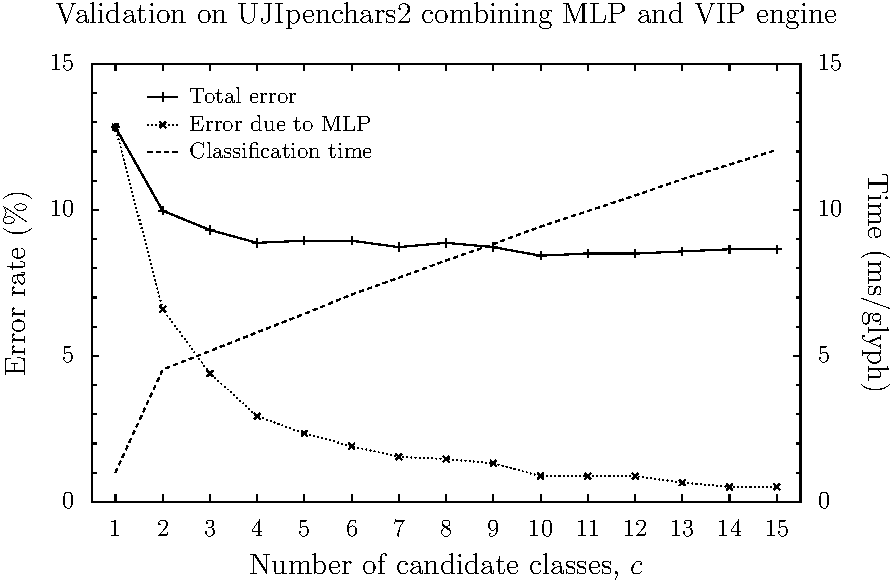
\includegraphics[width=\columnwidth]{Graphs/mlp_vip_UJIpenchars2.pdf}
  \hfill{}
  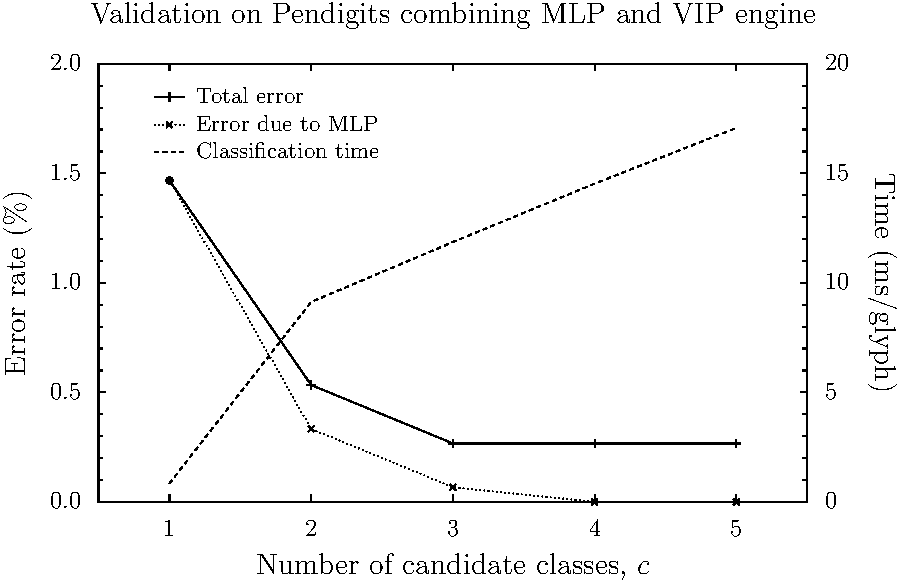
\includegraphics[width=\columnwidth]{Graphs/mlp_vip_Pendigits.pdf}
  \caption{Experimental results for choosing how many candidate classes the MLP must select.}
  \label{fig:choosing}
\end{figure*}

\SubSection{The databases}

We have experimented with two different databases of on-line isolated
handwritten characters: UJIpenchars2 and Pendigits.

\SubSubSection{UJIpenchars2}

This database~\cite{ujipenchars2}, available at the UCI Machine
Learning Repository~\cite{repository} and partially described
in~\cite{2008:lrec:llorens}, is an extension of
UJIpenchars~\cite{ujipenchars} containing instances of letters,
digits, and other symbols.

We have restricted ourselves to the $62$~ASCII alphanumeric
characters, which have been divided into~$35$ classes: $9$
for the ``1'' to ``9'' digits and $26$ for the lower and uppercase
versions of each letter, where zero is included in the ``o'' class.
In total, we have $4\,960$ training samples from $40$ writers and
$2\,480$ test samples from $20$ different writers.

When needed, we have reserved $11$ training writers (the UJIpenchars
ones) for validation purposes, thus splitting the considered set of
samples into three subsets: TR (proper training set, $29$ writers,
$3\,596$ samples), VA (validation set, $11$ writers, $1\,364$
samples), and TS (test set, $20$ writers, $2\,480$ samples).

\SubSubSection{Pendigits}

The Pendigits database~\cite{pendigits} is also available at the UCI
Machine Learning Repository~\cite{repository}.  This corpus contains
handwritten instances of the $10$ digits from several writers: $7\,494$
glyphs from $30$ writers are used as training set and $3\,498$ glyphs
from $14$ different writers are used as test data. Recently published
error rates over this database are $2.26\%$ in 2005~\cite{zhang05} and
$1.66\%$ in 2006~\cite{spillman06}.

When needed, $6$ writers have been reserved for validation purposes,
producing the following partition: TR (proper training set, $24$
writers, $5\,995$ samples), VA (validation set, $6$ writers, $1\,499$
samples), and TS (test set, $14$ writers, $3\,498$ samples).

\SubSection{MLP training for UJIpenchars2}

For training the MLPs, we have applied the on-line backpropagation
algorithm with momentum (see chapters~7 and~8 in~\cite{rojas96}) to
the cross-entropy penalty function~\cite{dunne97} measured on the
corresponding TR set. However, to avoid overfitting, the
stopping criterion does not take the TR set into account. Instead, the
training stops when the classification error on a subset of VA
does not improve for $100$ epochs. Then, the MLP from the epoch with
the minimum classification error so far is chosen.

In this work, all the MLP training has been carried out using the
\April{} toolkit~\cite{espana07} with scripts that include a
small decay to be applied to both learning rate and momentum after
each training epoch (they are multiplied by $0.999$).

As said before, just a subset of VA is employed for stopping the
training of each MLP. This subset, VA1, consists of $774$ samples from
$6$ writers. The remaining $620$ validation samples, from $5$ writers,
forms VA2. The classification error on this second validation set has
been used for choosing the best MLP among the networks returned for a number
of training runs.

All possible combinations of the following parameter values have been
tried in a first round of $2\,640$ runs (one run per parameter combination):
\begin{description}
  \item[Resampling sizes:] $10$, $20$, $30$, \ldots{}, $200$.

  \item[Grid sizes:] $3\times{}3$, $4\times{}4$, and $5\times{}5$.

  \item[Hidden layer topologies:] One layer with $32$, $64$, $96$, and $128$
  units and two layers with sizes $(32,32)$, $(64,32)$,
  $(96,32)$, $(128,32)$, $(64,64)$, $(96,64)$, and $(128,64)$.

  \item[Initial weight ranges:] Only $[-0.7,0.7]$.

  \item[Learning rate and momentum pairs:] $(0.05,0.01)$,
  $(0.01,0.002)$, $(0.075,0.025)$, and $(0.005,0.0001)$.
\end{description}

Then, for the three parameter combinations showing the best results on
VA2, a second round of training runs was performed varying the initial
weight range. Three intervals ($[-0.1,0.1]$, $[-0.4,0.4]$, and
$[-0.7,0.7]$) were considered for each parameter combination and ten
different MLPs were trained in each case, totalling $90$ new runs. It
is worth noting that, in each run, randomness affects both initial
weight values and the TR set shuffle before each epoch.

The network finally selected for the UJIpenchars2 task, which
achieves a $13.0\%$ error rate on VA2, is an MLP with $128$ units in
just one hidden layer, trained from weights initialized in the range
$[-0.1,0.1]$ with learning rate $0.05$, momentum $0.01$, and input
patterns obtained from a $4\times{}4$ grid after a $70$-segment
resampling of the preprocessed glyphs.

%%UJIPENCHARS2:
%%cheeses4-m070-128-pjsz0-lr0.050-mt0.010-s10-ir0.1.log
%%final best net: epoch 28
%%stop_val err =  12.581 choose val. error  13.038 N= 1
%%stop_val err =   6.129 choose val. error   6.989 N= 2
%%stop_val err =   4.194 choose val. error   4.570 N= 3
%%stop_val err =   3.387 choose val. error   2.554 N= 4
%%stop_val err =   2.419 choose val. error   2.285 N= 5

\SubSection{MLP training for Pendigits}

The same three parameter combinations selected after the first round
of runs in the previous section were used for training $90$ MLPs for
the new task, following the same process described above, except for
the fact that there is only one validation set, VA, to be used for
both the stopping criterion and choosing the best MLP.

The best performance is achieved by an MLP with two hidden layers
$(128,64)$, learning rate $0.05$, momentum $0.01$, initial weights in
the range $[-0.7,0.7]$, and input patterns obtained from a $3\times{}3$
grid after a $50$-segment resampling.  The classification error rate
for the validation set with this MLP is $1.47\%$.

%%PENDIGITS:
%%cheeses3-m050-128_64-pjsz0-lr0.050-mt0.010-s9-ir0.7.log
%%final best net: epoch 7
%%validation error 1.467645 N=1
%%validation error 0.333556 N=2
%%validation error 0.066711 N=3
%%validation error 0.000000 N=4
%%validation error 0.000000 N=5 

%------------------------------------------------------------------------- 
\SubSection{Choosing the number of candidate classes}

In order to choose the number $c$ of candidate classes the
corresponding MLP should provide to the VIP engine, new experiments
were carried out for both UJIpenchars2 and Pendigits. In each case, we
use the best MLP previously trained and, as prototypes for the VIP
engine, the corresponding TR set. Classification results, measured on
the corresponding complete VA set, are shown in
\CallOutOneFig{fig:choosing} for a range of $c$ values. The times
correspond to executions on a Dell Precision T3400 desktop PC with an
Intel Core2 Quad CPU Q9450 at $2.66$~GHz and $4$~Gb of RAM on the .NET
3.5 (with SP1) platform under the Microsoft Vista Ultimate Edition
(with SP1) operating system. The programs were coded in C\# without
unsafe code and compiled on Microsoft Visual Studio 2008 (with SP1).

Our final choice, minimizing classification errors, was $c=10$ for
UJIpenchars2 and $c=3$ for Pendigits, ie approximately one third of
the total number of classes in each case.

%------------------------------------------------------------------------- 
\SubSection{Comparative results}

\newcommand{\tbf}[1]{\textbf{#1}}
\begin{table*}[t]
  \caption{Classification error and running time per glyph (ms) on
  UJIpenchars2 and Pendigits.}\bigskip
  \centering
  \begin{tabular}{lrrrrrrrr}\toprule
    & \multicolumn{4}{c}{UJIpenchars2} & 
      \multicolumn{4}{c}{Pendigits} \\\cmidrule(r){2-5}\cmidrule(l){6-9}
    & \multicolumn{2}{c}{Validation} & \multicolumn{2}{c}{Test} &
      \multicolumn{2}{c}{Validation} & \multicolumn{2}{c}{Test} \\\midrule
Microsoft SDK &  8.4\% &  0.6 &      8.5\% & \tbf{0.6}& 0.93\% &  0.5 &      1.89\% & \tbf{0.5}\\
VIP engine    &  8.7\% & 16.7 &      8.5\% &     23.6 & 0.27\% & 26.0 & \tbf{0.60\%}&     32.4 \\
MLP           & 12.8\% &  1.0 &     14.2\% &      1.0 & 1.47\% &  0.8 &      3.63\% &      0.8 \\
MLP + VIP     &  8.4\% &  9.4 & \tbf{8.2\%}&     12.4 & 0.27\% & 11.9 &      0.80\% &     14.8 \\
\bottomrule
  \end{tabular}
  \label{tab:exps}
\end{table*}

Comparative results are presented in \CallOutOneTable{tab:exps}.
The first row corresponds to C\# experiments with the 1.7 version of the
Microsoft Tablet PC SDK recognition engine\footnote{In these
experiments, the Microsoft recognition engine uses a
\code{Microsoft.Ink.RecognizerContext} object with an appropriate
\code{WordList} and flags \code{Coerce} and \code{WordMode}. We also
help the Microsoft recognizer by providing it with the dimensions of
the acquisition box via its \code{Guide} property.}. The following
rows correspond to the engines explained above, using the same two
MLPs as in the previous section. In Validation columns,
classification is measured on VA sets and TR sets are used as VIP
prototypes. In Test columns, final results on TS sets are shown where,
when needed, complete training sets \mbox{TR + VA} are used by the VIP
engine.

The main result is that running time has been reduced to 50\% from the
baseline without significantly altering the error rate: the difference
is $0.20\%$ on Pendigits and $0.3\%$ on UJIpenchars2. On UJIpenchars2,
the \mbox{MLP + VIP} error rate ($8.2\%$) is clearly competitive with the
Microsoft engine ($8.5\%$), while in Pendigits, the error rates of VIP
($0.60\%$) and \mbox{MLP + VIP} ($0.80\%$) are definitely better than those of
Microsoft ($1.89\%$).

%------------------------------------------------------------------------- 
\Section{Conclusions}
\label{sec:conclusions}

The integration of MLPs into our engine approximately halves its
running time while keeping the error rates. Compared to the Microsoft
engine, the results are competitive and our code is completely
managed, so it can be ported to any architecture running a .NET
platform, like Windows, Linux, and Mac~OS~X, among others.

The current times correspond to more than 60 characters per second,
making it suitable for real-time response.

%------------------------------------------------------------------------- 
\UnnumberedSection{Acknowledgments}

Work partially supported by the Spanish \emph{Ministerio de Ciencia e
Innovaci�n} (TIN2006-12767, TIN2008-06856, and \emph{Consolider Ingenio 2010}
CSD2007-00018), the \emph{Conselleria d'Empresa, Universitat i
Ci�ncia, Generalitat Valenciana} (BFPI06/250 scholarship), and
\emph{Fundaci� Caixa Castell�-Bancaixa} (P1$\cdot$1B2006-31).

\bibliographystyle{../latex8}
\bibliography{../icdar09}

\end{document}

%%% Local Variables:
%%% mode: latex
%%% TeX-master: t
%%% ispell-local-dictionary: "american"
%%% End:
